% Options for packages loaded elsewhere
\PassOptionsToPackage{unicode}{hyperref}
\PassOptionsToPackage{hyphens}{url}
%
\documentclass[
]{article}
\usepackage{amsmath,amssymb}
\usepackage{lmodern}
\usepackage{ifxetex,ifluatex}
\ifnum 0\ifxetex 1\fi\ifluatex 1\fi=0 % if pdftex
  \usepackage[T1]{fontenc}
  \usepackage[utf8]{inputenc}
  \usepackage{textcomp} % provide euro and other symbols
\else % if luatex or xetex
  \usepackage{unicode-math}
  \defaultfontfeatures{Scale=MatchLowercase}
  \defaultfontfeatures[\rmfamily]{Ligatures=TeX,Scale=1}
\fi
% Use upquote if available, for straight quotes in verbatim environments
\IfFileExists{upquote.sty}{\usepackage{upquote}}{}
\IfFileExists{microtype.sty}{% use microtype if available
  \usepackage[]{microtype}
  \UseMicrotypeSet[protrusion]{basicmath} % disable protrusion for tt fonts
}{}
\makeatletter
\@ifundefined{KOMAClassName}{% if non-KOMA class
  \IfFileExists{parskip.sty}{%
    \usepackage{parskip}
  }{% else
    \setlength{\parindent}{0pt}
    \setlength{\parskip}{6pt plus 2pt minus 1pt}}
}{% if KOMA class
  \KOMAoptions{parskip=half}}
\makeatother
\usepackage{xcolor}
\IfFileExists{xurl.sty}{\usepackage{xurl}}{} % add URL line breaks if available
\IfFileExists{bookmark.sty}{\usepackage{bookmark}}{\usepackage{hyperref}}
\hypersetup{
  pdftitle={P8130\_hw2\_wq2160},
  pdfauthor={Wenshan Qu (wq2160)},
  hidelinks,
  pdfcreator={LaTeX via pandoc}}
\urlstyle{same} % disable monospaced font for URLs
\usepackage[margin=1in]{geometry}
\usepackage{color}
\usepackage{fancyvrb}
\newcommand{\VerbBar}{|}
\newcommand{\VERB}{\Verb[commandchars=\\\{\}]}
\DefineVerbatimEnvironment{Highlighting}{Verbatim}{commandchars=\\\{\}}
% Add ',fontsize=\small' for more characters per line
\usepackage{framed}
\definecolor{shadecolor}{RGB}{248,248,248}
\newenvironment{Shaded}{\begin{snugshade}}{\end{snugshade}}
\newcommand{\AlertTok}[1]{\textcolor[rgb]{0.94,0.16,0.16}{#1}}
\newcommand{\AnnotationTok}[1]{\textcolor[rgb]{0.56,0.35,0.01}{\textbf{\textit{#1}}}}
\newcommand{\AttributeTok}[1]{\textcolor[rgb]{0.77,0.63,0.00}{#1}}
\newcommand{\BaseNTok}[1]{\textcolor[rgb]{0.00,0.00,0.81}{#1}}
\newcommand{\BuiltInTok}[1]{#1}
\newcommand{\CharTok}[1]{\textcolor[rgb]{0.31,0.60,0.02}{#1}}
\newcommand{\CommentTok}[1]{\textcolor[rgb]{0.56,0.35,0.01}{\textit{#1}}}
\newcommand{\CommentVarTok}[1]{\textcolor[rgb]{0.56,0.35,0.01}{\textbf{\textit{#1}}}}
\newcommand{\ConstantTok}[1]{\textcolor[rgb]{0.00,0.00,0.00}{#1}}
\newcommand{\ControlFlowTok}[1]{\textcolor[rgb]{0.13,0.29,0.53}{\textbf{#1}}}
\newcommand{\DataTypeTok}[1]{\textcolor[rgb]{0.13,0.29,0.53}{#1}}
\newcommand{\DecValTok}[1]{\textcolor[rgb]{0.00,0.00,0.81}{#1}}
\newcommand{\DocumentationTok}[1]{\textcolor[rgb]{0.56,0.35,0.01}{\textbf{\textit{#1}}}}
\newcommand{\ErrorTok}[1]{\textcolor[rgb]{0.64,0.00,0.00}{\textbf{#1}}}
\newcommand{\ExtensionTok}[1]{#1}
\newcommand{\FloatTok}[1]{\textcolor[rgb]{0.00,0.00,0.81}{#1}}
\newcommand{\FunctionTok}[1]{\textcolor[rgb]{0.00,0.00,0.00}{#1}}
\newcommand{\ImportTok}[1]{#1}
\newcommand{\InformationTok}[1]{\textcolor[rgb]{0.56,0.35,0.01}{\textbf{\textit{#1}}}}
\newcommand{\KeywordTok}[1]{\textcolor[rgb]{0.13,0.29,0.53}{\textbf{#1}}}
\newcommand{\NormalTok}[1]{#1}
\newcommand{\OperatorTok}[1]{\textcolor[rgb]{0.81,0.36,0.00}{\textbf{#1}}}
\newcommand{\OtherTok}[1]{\textcolor[rgb]{0.56,0.35,0.01}{#1}}
\newcommand{\PreprocessorTok}[1]{\textcolor[rgb]{0.56,0.35,0.01}{\textit{#1}}}
\newcommand{\RegionMarkerTok}[1]{#1}
\newcommand{\SpecialCharTok}[1]{\textcolor[rgb]{0.00,0.00,0.00}{#1}}
\newcommand{\SpecialStringTok}[1]{\textcolor[rgb]{0.31,0.60,0.02}{#1}}
\newcommand{\StringTok}[1]{\textcolor[rgb]{0.31,0.60,0.02}{#1}}
\newcommand{\VariableTok}[1]{\textcolor[rgb]{0.00,0.00,0.00}{#1}}
\newcommand{\VerbatimStringTok}[1]{\textcolor[rgb]{0.31,0.60,0.02}{#1}}
\newcommand{\WarningTok}[1]{\textcolor[rgb]{0.56,0.35,0.01}{\textbf{\textit{#1}}}}
\usepackage{graphicx}
\makeatletter
\def\maxwidth{\ifdim\Gin@nat@width>\linewidth\linewidth\else\Gin@nat@width\fi}
\def\maxheight{\ifdim\Gin@nat@height>\textheight\textheight\else\Gin@nat@height\fi}
\makeatother
% Scale images if necessary, so that they will not overflow the page
% margins by default, and it is still possible to overwrite the defaults
% using explicit options in \includegraphics[width, height, ...]{}
\setkeys{Gin}{width=\maxwidth,height=\maxheight,keepaspectratio}
% Set default figure placement to htbp
\makeatletter
\def\fps@figure{htbp}
\makeatother
\setlength{\emergencystretch}{3em} % prevent overfull lines
\providecommand{\tightlist}{%
  \setlength{\itemsep}{0pt}\setlength{\parskip}{0pt}}
\setcounter{secnumdepth}{-\maxdimen} % remove section numbering
\ifluatex
  \usepackage{selnolig}  % disable illegal ligatures
\fi

\title{P8130\_hw2\_wq2160}
\author{Wenshan Qu (wq2160)}
\date{}

\begin{document}
\maketitle

\hypertarget{problem-1}{%
\subsection{Problem 1}\label{problem-1}}

Draw a random sample without replacement of 200 observations (100 men
and 100 women) from the entire CE data set named ce8130entire.csv. Call
this first sample ``A'' and save the sample. In ``sex'' variable,
\textbf{men} are identified by \textbf{``1''}, and \textbf{women} by
\textbf{``2''}. Note: To obtain the sample data set of approximately 200
observations, you can use the following code. Replace the ``set.seed''
number with an integer of your choice (3 points).

\begin{Shaded}
\begin{Highlighting}[]
\NormalTok{population }\OtherTok{=} \FunctionTok{read.csv}\NormalTok{(}\StringTok{"./ce8130entire.csv"}\NormalTok{)}

\FunctionTok{set.seed}\NormalTok{(}\DecValTok{33}\NormalTok{)}
\NormalTok{A }\OtherTok{=} 
\NormalTok{  population }\SpecialCharTok{\%\textgreater{}\%} 
  \FunctionTok{group\_by}\NormalTok{(sex) }\SpecialCharTok{\%\textgreater{}\%} 
  \FunctionTok{sample\_n}\NormalTok{(}\DecValTok{100}\NormalTok{)}

\NormalTok{A}
\end{Highlighting}
\end{Shaded}

\begin{verbatim}
## # A tibble: 200 x 7
## # Groups:   sex [2]
##    provnum   sex  race smoker totchg   age  year
##      <int> <int> <int>  <int>  <int> <int> <int>
##  1      28     1     0      0  13434    78  1995
##  2      21     1     0      0   7701    60  1995
##  3       7     1     0      0   2225    67  1991
##  4      20     1     0      0   8369    68  1994
##  5      47     1     0      0   3095    77  1992
##  6       7     1     0      0   4134    68  1992
##  7      14     1     0      0   3226    63  1992
##  8      27     1     0      0   4592    71  1992
##  9      48     1     0      0   4988    60  1993
## 10      14     1     0      0   5180    68  1994
## # ... with 190 more rows
\end{verbatim}

\hypertarget{problem-2}{%
\subsection{Problem 2}\label{problem-2}}

Now use the same seed as before but this time draw a random sample
without replacement of 60 observations (30 men and 30 women) and call it
sample ``B'' (Note that Sample ``B'' is more than 3 times smaller than
sample ``A''). Save it as a separate sample. Replace the seed number
with the same seed number as you used above (3 points).

\begin{Shaded}
\begin{Highlighting}[]
\FunctionTok{set.seed}\NormalTok{(}\DecValTok{33}\NormalTok{)}
\NormalTok{B }\OtherTok{=} 
\NormalTok{  population }\SpecialCharTok{\%\textgreater{}\%} 
  \FunctionTok{group\_by}\NormalTok{(sex) }\SpecialCharTok{\%\textgreater{}\%} 
  \FunctionTok{sample\_n}\NormalTok{(}\DecValTok{30}\NormalTok{)}

\NormalTok{B}
\end{Highlighting}
\end{Shaded}

\begin{verbatim}
## # A tibble: 60 x 7
## # Groups:   sex [2]
##    provnum   sex  race smoker totchg   age  year
##      <int> <int> <int>  <int>  <int> <int> <int>
##  1      28     1     0      0  13434    78  1995
##  2      21     1     0      0   7701    60  1995
##  3       7     1     0      0   2225    67  1991
##  4      20     1     0      0   8369    68  1994
##  5      47     1     0      0   3095    77  1992
##  6       7     1     0      0   4134    68  1992
##  7      14     1     0      0   3226    63  1992
##  8      27     1     0      0   4592    71  1992
##  9      48     1     0      0   4988    60  1993
## 10      14     1     0      0   5180    68  1994
## # ... with 50 more rows
\end{verbatim}

\hypertarget{problem-3}{%
\subsection{Problem 3}\label{problem-3}}

Using sample ``A'', display the distribution of CE cost in \$USD
(variable name: ``totchg'') separately for men and women using
side-by-side boxplots and histograms. Label your figures appropriately.

\textbf{Histogram}

\begin{Shaded}
\begin{Highlighting}[]
\NormalTok{hist\_plot }\OtherTok{=} 
\NormalTok{A }\SpecialCharTok{\%\textgreater{}\%} 
  \FunctionTok{mutate}\NormalTok{(}\AttributeTok{sex =} \FunctionTok{recode}\NormalTok{(sex, }\StringTok{"1"} \OtherTok{=} \StringTok{"men"}\NormalTok{, }\StringTok{"2"} \OtherTok{=} \StringTok{"women"}\NormalTok{)) }\SpecialCharTok{\%\textgreater{}\%} 
  \FunctionTok{ggplot}\NormalTok{(}\FunctionTok{aes}\NormalTok{(}\AttributeTok{x =}\NormalTok{ totchg)) }\SpecialCharTok{+}
  \FunctionTok{geom\_histogram}\NormalTok{() }\SpecialCharTok{+}
  \FunctionTok{facet\_grid}\NormalTok{(. }\SpecialCharTok{\textasciitilde{}}\NormalTok{ sex) }\SpecialCharTok{+}
  \FunctionTok{labs}\NormalTok{(}
    \AttributeTok{title =} \StringTok{"The Distribution of CE Cost (Histogram)"}\NormalTok{,}
    \AttributeTok{subtitle =} \StringTok{"Separately for Men and Women"}\NormalTok{,}
    \AttributeTok{x =} \StringTok{"CE cost ($USD)"}\NormalTok{,}
    \AttributeTok{y =} \StringTok{"Frequency"}
\NormalTok{  ) }\SpecialCharTok{+}
  \FunctionTok{theme\_bw}\NormalTok{()}

\NormalTok{hist\_plot}
\end{Highlighting}
\end{Shaded}

\begin{verbatim}
## `stat_bin()` using `bins = 30`. Pick better value with `binwidth`.
\end{verbatim}

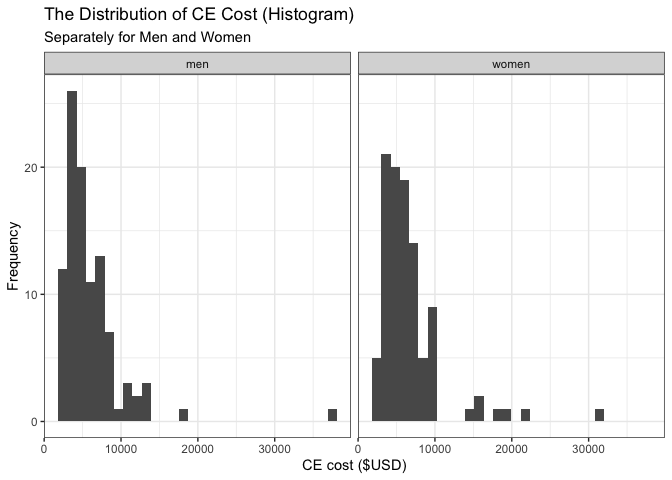
\includegraphics{P8130_hw3_wq2160_files/figure-latex/unnamed-chunk-4-1.pdf}

\textbf{Boxplot}

\begin{Shaded}
\begin{Highlighting}[]
\NormalTok{boxp\_plot }\OtherTok{=} 
\NormalTok{A }\SpecialCharTok{\%\textgreater{}\%} 
  \FunctionTok{mutate}\NormalTok{(}\AttributeTok{sex =} \FunctionTok{recode}\NormalTok{(sex, }\StringTok{"1"} \OtherTok{=} \StringTok{"men"}\NormalTok{, }\StringTok{"2"} \OtherTok{=} \StringTok{"women"}\NormalTok{)) }\SpecialCharTok{\%\textgreater{}\%} 
  \FunctionTok{ggplot}\NormalTok{(}\FunctionTok{aes}\NormalTok{(}\AttributeTok{x =}\NormalTok{ sex, }\AttributeTok{y =}\NormalTok{ totchg)) }\SpecialCharTok{+}
  \FunctionTok{geom\_boxplot}\NormalTok{() }\SpecialCharTok{+}
  \FunctionTok{labs}\NormalTok{(}
    \AttributeTok{title =} \StringTok{"The Distribution of CE Cost (Boxplot)"}\NormalTok{,}
    \AttributeTok{subtitle =} \StringTok{"Separately for Men and Women"}\NormalTok{,}
    \AttributeTok{x =} \StringTok{"Sex"}\NormalTok{,}
    \AttributeTok{y =} \StringTok{"CE cost ($USD)"}
\NormalTok{  ) }\SpecialCharTok{+}
  \FunctionTok{scale\_y\_continuous}\NormalTok{(}
    \AttributeTok{breaks =} \FunctionTok{c}\NormalTok{(}\DecValTok{5000}\NormalTok{, }\DecValTok{10000}\NormalTok{, }\DecValTok{15000}\NormalTok{, }\DecValTok{20000}\NormalTok{, }\DecValTok{25000}\NormalTok{, }\DecValTok{30000}\NormalTok{),}
    \AttributeTok{labels =} \FunctionTok{c}\NormalTok{(}\StringTok{"5000"}\NormalTok{, }\StringTok{"10000"}\NormalTok{, }\StringTok{"15000"}\NormalTok{, }\StringTok{"20000"}\NormalTok{, }\StringTok{"25000"}\NormalTok{, }\StringTok{"30000"}\NormalTok{)}
\NormalTok{  ) }\SpecialCharTok{+}
  \FunctionTok{theme\_bw}\NormalTok{()}

\NormalTok{boxp\_plot}
\end{Highlighting}
\end{Shaded}

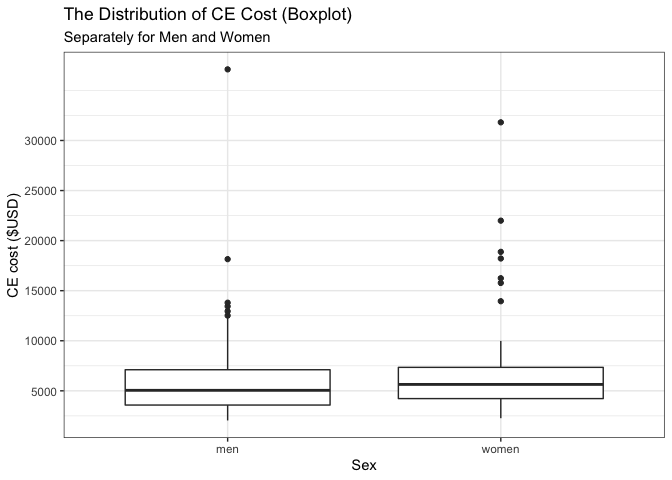
\includegraphics{P8130_hw3_wq2160_files/figure-latex/unnamed-chunk-5-1.pdf}

\hypertarget{problem-4}{%
\subsection{Problem 4}\label{problem-4}}

Calculate the mean CE cost and 95\% confidence interval separately for
men and women in sample ``A'' as well as sample ``B''. Assume we don't
know the population variance. Plot the sample ``A'' and sample ``B''
confidence intervals next to each other (by sex). How do they differ,
which confidence intervals are wider? Explain why. \#\#Note: For the
purposes of confidence interval estimation and hypothesis testing, let's
assume that all the assumptions, including the assumption of normal
distribution, are met.

\hypertarget{plot-sample-a-and-b-ci}{%
\paragraph{4.1 Plot sample A and B CI}\label{plot-sample-a-and-b-ci}}

\begin{Shaded}
\begin{Highlighting}[]
\NormalTok{A\_s }\OtherTok{=} 
\NormalTok{  A }\SpecialCharTok{\%\textgreater{}\%} 
  \FunctionTok{mutate}\NormalTok{(}\AttributeTok{sample =} \FunctionTok{c}\NormalTok{(}\StringTok{"Sample A"}\NormalTok{))}

\NormalTok{B\_s }\OtherTok{=} 
\NormalTok{  B }\SpecialCharTok{\%\textgreater{}\%} 
  \FunctionTok{mutate}\NormalTok{(}\AttributeTok{sample =} \FunctionTok{c}\NormalTok{(}\StringTok{"Sample B"}\NormalTok{))}

\NormalTok{AB\_df }\OtherTok{=} \FunctionTok{rbind}\NormalTok{(A\_s, B\_s)}

\NormalTok{p\_dodge }\OtherTok{=} \FunctionTok{position\_dodge}\NormalTok{(}\FloatTok{0.1}\NormalTok{)}

\NormalTok{AB\_plot }\OtherTok{=} 
\NormalTok{AB\_df }\SpecialCharTok{\%\textgreater{}\%} 
  \FunctionTok{mutate}\NormalTok{(}\AttributeTok{sex =} \FunctionTok{recode}\NormalTok{(sex, }\StringTok{"1"} \OtherTok{=} \StringTok{"men"}\NormalTok{, }\StringTok{"2"} \OtherTok{=} \StringTok{"women"}\NormalTok{)) }\SpecialCharTok{\%\textgreater{}\%} 
  \FunctionTok{summarySE}\NormalTok{(}\AttributeTok{measurevar =} \StringTok{"totchg"}\NormalTok{, }\AttributeTok{groupvars =} \FunctionTok{c}\NormalTok{(}\StringTok{"sex"}\NormalTok{, }\StringTok{"sample"}\NormalTok{)) }\SpecialCharTok{\%\textgreater{}\%} 
  \FunctionTok{ggplot}\NormalTok{(}\FunctionTok{aes}\NormalTok{(}\AttributeTok{x =}\NormalTok{ sex, }\AttributeTok{y =}\NormalTok{ totchg, }\AttributeTok{color =}\NormalTok{ sex)) }\SpecialCharTok{+}
  \FunctionTok{geom\_point}\NormalTok{() }\SpecialCharTok{+}
  \FunctionTok{geom\_errorbar}\NormalTok{(}\FunctionTok{aes}\NormalTok{(}\AttributeTok{ymin =}\NormalTok{ totchg }\SpecialCharTok{{-}}\NormalTok{ ci, }\AttributeTok{ymax =}\NormalTok{ totchg }\SpecialCharTok{+}\NormalTok{ ci), }\AttributeTok{width =}\NormalTok{ .}\DecValTok{1}\NormalTok{, }\AttributeTok{position =}\NormalTok{ p\_dodge) }\SpecialCharTok{+}
  \FunctionTok{facet\_grid}\NormalTok{(. }\SpecialCharTok{\textasciitilde{}}\NormalTok{ sample) }\SpecialCharTok{+}
  \FunctionTok{labs}\NormalTok{(}
    \AttributeTok{title =} \StringTok{"The CI of Sample A and Sample B"}\NormalTok{,}
    \AttributeTok{subtitle =} \StringTok{"Separate by Sex"}\NormalTok{,}
    \AttributeTok{x =} \StringTok{"Sex"}\NormalTok{,}
    \AttributeTok{y =} \StringTok{"Total Charge"}
\NormalTok{  ) }\SpecialCharTok{+}
  \FunctionTok{theme\_bw}\NormalTok{() }\SpecialCharTok{+}
  \FunctionTok{theme}\NormalTok{(}\AttributeTok{legend.position =} \StringTok{"none"}\NormalTok{)}

\NormalTok{AB\_plot}
\end{Highlighting}
\end{Shaded}

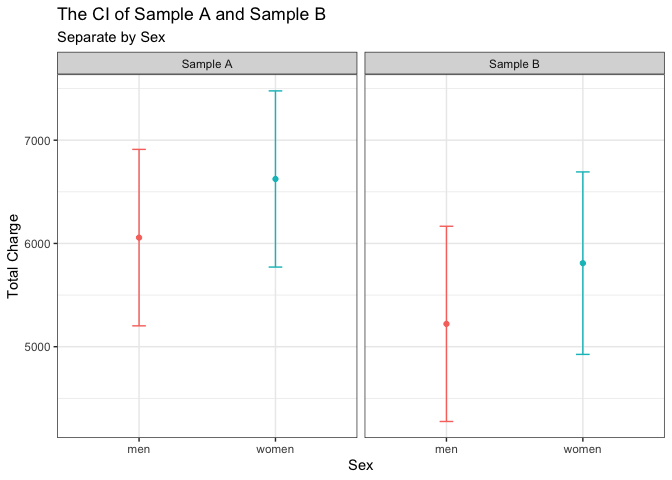
\includegraphics{P8130_hw3_wq2160_files/figure-latex/unnamed-chunk-6-1.pdf}

\hypertarget{manually-calculation-for-sample-a}{%
\paragraph{4.2 Manually calculation for Sample
A}\label{manually-calculation-for-sample-a}}

\textbf{mean CE cost and 95\% confidence interval for MEN}

\begin{Shaded}
\begin{Highlighting}[]
\NormalTok{A\_men }\OtherTok{=} 
\NormalTok{A }\SpecialCharTok{\%\textgreater{}\%} 
  \FunctionTok{filter}\NormalTok{(sex }\SpecialCharTok{==} \StringTok{"1"}\NormalTok{)}

\DocumentationTok{\#\# Mean CE cost for MEN}
\NormalTok{mean1 }\OtherTok{=} 
\NormalTok{A\_men }\SpecialCharTok{\%\textgreater{}\%} 
  \FunctionTok{summarize}\NormalTok{(}\AttributeTok{mean\_cost\_men =} \FunctionTok{mean}\NormalTok{(totchg)) }

\NormalTok{mean1}
\end{Highlighting}
\end{Shaded}

\begin{verbatim}
##   mean_cost_men
## 1       6056.47
\end{verbatim}

\begin{Shaded}
\begin{Highlighting}[]
\DocumentationTok{\#\# 95\% CI for MEN}
\NormalTok{x1 }\OtherTok{=} \FunctionTok{mean}\NormalTok{(}\FunctionTok{pull}\NormalTok{(A\_men, totchg))}
\NormalTok{s1 }\OtherTok{=} \FunctionTok{sd}\NormalTok{(}\FunctionTok{pull}\NormalTok{(A\_men, totchg))}
\NormalTok{n1 }\OtherTok{=} \DecValTok{100}
\NormalTok{t1 }\OtherTok{=} \FunctionTok{qt}\NormalTok{(}\FloatTok{0.975}\NormalTok{, }\AttributeTok{df =} \DecValTok{100} \SpecialCharTok{{-}} \DecValTok{1}\NormalTok{)}

\NormalTok{upper1 }\OtherTok{=}\NormalTok{ x1 }\SpecialCharTok{+}\NormalTok{ t1 }\SpecialCharTok{*}\NormalTok{ s1 }\SpecialCharTok{/} \FunctionTok{sqrt}\NormalTok{(n1)}
\NormalTok{lower1 }\OtherTok{=}\NormalTok{ x1 }\SpecialCharTok{{-}}\NormalTok{ t1 }\SpecialCharTok{*}\NormalTok{ s1 }\SpecialCharTok{/} \FunctionTok{sqrt}\NormalTok{(n1)}

\NormalTok{upper1}
\end{Highlighting}
\end{Shaded}

\begin{verbatim}
## [1] 6910.899
\end{verbatim}

\begin{Shaded}
\begin{Highlighting}[]
\NormalTok{lower1}
\end{Highlighting}
\end{Shaded}

\begin{verbatim}
## [1] 5202.041
\end{verbatim}

\textbf{mean CE cost and 95\% confidence interval for WOMEN}

\begin{Shaded}
\begin{Highlighting}[]
\NormalTok{A\_women }\OtherTok{=} 
\NormalTok{A }\SpecialCharTok{\%\textgreater{}\%} 
  \FunctionTok{filter}\NormalTok{(sex }\SpecialCharTok{==} \StringTok{"2"}\NormalTok{)}

\DocumentationTok{\#\# Mean CE cost for WOMEN}
\NormalTok{mean2 }\OtherTok{=} 
\NormalTok{A\_women }\SpecialCharTok{\%\textgreater{}\%} 
  \FunctionTok{summarize}\NormalTok{(}\AttributeTok{mean\_cost\_women =} \FunctionTok{mean}\NormalTok{(totchg)) }

\NormalTok{mean2}
\end{Highlighting}
\end{Shaded}

\begin{verbatim}
##   mean_cost_women
## 1         6624.28
\end{verbatim}

\begin{Shaded}
\begin{Highlighting}[]
\DocumentationTok{\#\# 95\% CI for WOMEN}
\NormalTok{x2 }\OtherTok{=} \FunctionTok{mean}\NormalTok{(}\FunctionTok{pull}\NormalTok{(A\_women, totchg))}
\NormalTok{s2 }\OtherTok{=} \FunctionTok{sd}\NormalTok{(}\FunctionTok{pull}\NormalTok{(A\_women, totchg))}
\NormalTok{n2 }\OtherTok{=} \DecValTok{100}
\NormalTok{t2 }\OtherTok{=} \FunctionTok{qt}\NormalTok{(}\FloatTok{0.975}\NormalTok{, }\AttributeTok{df =} \DecValTok{100} \SpecialCharTok{{-}} \DecValTok{1}\NormalTok{)}

\NormalTok{upper2 }\OtherTok{=}\NormalTok{ x2 }\SpecialCharTok{+}\NormalTok{ t2 }\SpecialCharTok{*}\NormalTok{ s2 }\SpecialCharTok{/} \FunctionTok{sqrt}\NormalTok{(n2)}
\NormalTok{lower2 }\OtherTok{=}\NormalTok{ x2 }\SpecialCharTok{{-}}\NormalTok{ t2 }\SpecialCharTok{*}\NormalTok{ s2 }\SpecialCharTok{/} \FunctionTok{sqrt}\NormalTok{(n2)}

\NormalTok{upper2}
\end{Highlighting}
\end{Shaded}

\begin{verbatim}
## [1] 7477.367
\end{verbatim}

\begin{Shaded}
\begin{Highlighting}[]
\NormalTok{lower2}
\end{Highlighting}
\end{Shaded}

\begin{verbatim}
## [1] 5771.193
\end{verbatim}

\hypertarget{manually-calculation-for-sample-b}{%
\paragraph{4.3 Manually calculation for Sample
B}\label{manually-calculation-for-sample-b}}

\textbf{mean CE cost and 95\% confidence interval for MEN}

\begin{Shaded}
\begin{Highlighting}[]
\NormalTok{B\_men }\OtherTok{=} 
\NormalTok{B }\SpecialCharTok{\%\textgreater{}\%} 
  \FunctionTok{filter}\NormalTok{(sex }\SpecialCharTok{==} \StringTok{"1"}\NormalTok{)}

\DocumentationTok{\#\# Mean CE cost for MEN}
\NormalTok{mean3 }\OtherTok{=} 
\NormalTok{B\_men }\SpecialCharTok{\%\textgreater{}\%} 
  \FunctionTok{summarize}\NormalTok{(}\AttributeTok{mean\_cost\_men =} \FunctionTok{mean}\NormalTok{(totchg)) }

\NormalTok{mean3}
\end{Highlighting}
\end{Shaded}

\begin{verbatim}
##   mean_cost_men
## 1      5221.133
\end{verbatim}

\begin{Shaded}
\begin{Highlighting}[]
\DocumentationTok{\#\# 95\% CI for MEN}
\NormalTok{x3 }\OtherTok{=} \FunctionTok{mean}\NormalTok{(}\FunctionTok{pull}\NormalTok{(B\_men, totchg))}
\NormalTok{s3 }\OtherTok{=} \FunctionTok{sd}\NormalTok{(}\FunctionTok{pull}\NormalTok{(B\_men, totchg))}
\NormalTok{n3 }\OtherTok{=} \DecValTok{30}
\NormalTok{t3 }\OtherTok{=} \FunctionTok{qt}\NormalTok{(}\FloatTok{0.975}\NormalTok{, }\AttributeTok{df =} \DecValTok{30} \SpecialCharTok{{-}} \DecValTok{1}\NormalTok{)}

\NormalTok{upper3 }\OtherTok{=}\NormalTok{ x3 }\SpecialCharTok{+}\NormalTok{ t3 }\SpecialCharTok{*}\NormalTok{ s3 }\SpecialCharTok{/} \FunctionTok{sqrt}\NormalTok{(n3)}
\NormalTok{lower3 }\OtherTok{=}\NormalTok{ x3 }\SpecialCharTok{{-}}\NormalTok{ t3 }\SpecialCharTok{*}\NormalTok{ s3 }\SpecialCharTok{/} \FunctionTok{sqrt}\NormalTok{(n3)}

\NormalTok{upper3}
\end{Highlighting}
\end{Shaded}

\begin{verbatim}
## [1] 6166.488
\end{verbatim}

\begin{Shaded}
\begin{Highlighting}[]
\NormalTok{lower3}
\end{Highlighting}
\end{Shaded}

\begin{verbatim}
## [1] 4275.779
\end{verbatim}

\textbf{mean CE cost and 95\% confidence interval for WOMEN}

\begin{Shaded}
\begin{Highlighting}[]
\NormalTok{B\_women }\OtherTok{=} 
\NormalTok{B }\SpecialCharTok{\%\textgreater{}\%} 
  \FunctionTok{filter}\NormalTok{(sex }\SpecialCharTok{==} \StringTok{"2"}\NormalTok{)}

\DocumentationTok{\#\# Mean CE cost for WOMEN}
\NormalTok{mean4 }\OtherTok{=} 
\NormalTok{B\_women }\SpecialCharTok{\%\textgreater{}\%} 
  \FunctionTok{summarize}\NormalTok{(}\AttributeTok{mean\_cost\_women =} \FunctionTok{mean}\NormalTok{(totchg)) }

\NormalTok{mean2}
\end{Highlighting}
\end{Shaded}

\begin{verbatim}
##   mean_cost_women
## 1         6624.28
\end{verbatim}

\begin{Shaded}
\begin{Highlighting}[]
\DocumentationTok{\#\# 95\% CI for WOMEN}
\NormalTok{x4 }\OtherTok{=} \FunctionTok{mean}\NormalTok{(}\FunctionTok{pull}\NormalTok{(B\_women, totchg))}
\NormalTok{s4 }\OtherTok{=} \FunctionTok{sd}\NormalTok{(}\FunctionTok{pull}\NormalTok{(B\_women, totchg))}
\NormalTok{n4 }\OtherTok{=} \DecValTok{30}
\NormalTok{t4 }\OtherTok{=} \FunctionTok{qt}\NormalTok{(}\FloatTok{0.975}\NormalTok{, }\AttributeTok{df =} \DecValTok{30} \SpecialCharTok{{-}} \DecValTok{1}\NormalTok{)}

\NormalTok{upper4 }\OtherTok{=}\NormalTok{ x4 }\SpecialCharTok{+}\NormalTok{ t4 }\SpecialCharTok{*}\NormalTok{ s4 }\SpecialCharTok{/} \FunctionTok{sqrt}\NormalTok{(n4)}
\NormalTok{lower4 }\OtherTok{=}\NormalTok{ x4 }\SpecialCharTok{{-}}\NormalTok{ t4 }\SpecialCharTok{*}\NormalTok{ s4 }\SpecialCharTok{/} \FunctionTok{sqrt}\NormalTok{(n4)}

\NormalTok{upper4}
\end{Highlighting}
\end{Shaded}

\begin{verbatim}
## [1] 6692.608
\end{verbatim}

\begin{Shaded}
\begin{Highlighting}[]
\NormalTok{lower4}
\end{Highlighting}
\end{Shaded}

\begin{verbatim}
## [1] 4925.459
\end{verbatim}

Q1: How do they differ?

A1: There is a obvious trend that the mean CE cost of women is higher
than men in both samples, and this cost difference is about 570 USD.
(Note: According to Sample A and B.)

Q2: Which CI are wider?

A2: I think the CI width of two sample groups are nearly the same, and
the CI width of men and women in each sample group are also nearly the
same. According to calculation, in Sample A, the CI width of Men is
1708.86, of Women is 2273.98; in Sample B the CI width of Men is
1890.71, of Women is 1767.15. Consequently, there is no significant
difference exists.

Q3: Explain why?

A3: Sample A and B come from the same source population, then the total
``trend'' in these two samples should be nearly the same, which means
they are shows that 1) the CE cost of women is higher than men; and 2)
there is no significantly CI difference between women and men. However,
Sample A have a size of 200, Sample B only have 60 sample size, so the
latter one may more far away from the truth.

\begin{Shaded}
\begin{Highlighting}[]
\DocumentationTok{\#\# We can simply calculate the CI interval for each group}
\NormalTok{upper1}\SpecialCharTok{{-}}\NormalTok{lower1 }\DocumentationTok{\#\# Sample A Men}
\end{Highlighting}
\end{Shaded}

\begin{verbatim}
## [1] 1708.858
\end{verbatim}

\begin{Shaded}
\begin{Highlighting}[]
\NormalTok{upper2}\SpecialCharTok{{-}}\NormalTok{lower2 }\DocumentationTok{\#\# Sample A Women}
\end{Highlighting}
\end{Shaded}

\begin{verbatim}
## [1] 1706.173
\end{verbatim}

\begin{Shaded}
\begin{Highlighting}[]
\NormalTok{upper3}\SpecialCharTok{{-}}\NormalTok{lower3 }\DocumentationTok{\#\# Sample B Men}
\end{Highlighting}
\end{Shaded}

\begin{verbatim}
## [1] 1890.709
\end{verbatim}

\begin{Shaded}
\begin{Highlighting}[]
\NormalTok{upper4}\SpecialCharTok{{-}}\NormalTok{lower4 }\DocumentationTok{\#\# Sample B Women}
\end{Highlighting}
\end{Shaded}

\begin{verbatim}
## [1] 1767.149
\end{verbatim}

\hypertarget{problem-5}{%
\subsection{Problem 5}\label{problem-5}}

Conduct test of equality of variance of CE cost among men vs women in
sample A and interpret your results.

\textbf{Method 1}

\begin{Shaded}
\begin{Highlighting}[]
\FunctionTok{var.test}\NormalTok{(totchg }\SpecialCharTok{\textasciitilde{}}\NormalTok{ sex, }\AttributeTok{data =}\NormalTok{ A)}
\end{Highlighting}
\end{Shaded}

\begin{verbatim}
## 
##  F test to compare two variances
## 
## data:  totchg by sex
## F = 1.0031, num df = 99, denom df = 99, p-value = 0.9875
## alternative hypothesis: true ratio of variances is not equal to 1
## 95 percent confidence interval:
##  0.6749611 1.4909153
## sample estimates:
## ratio of variances 
##            1.00315
\end{verbatim}

\textbf{Method 2}

\begin{Shaded}
\begin{Highlighting}[]
\DocumentationTok{\#\# Test statistic for F test}
\NormalTok{F\_test }\OtherTok{=}\NormalTok{ s1}\SpecialCharTok{\^{}}\DecValTok{2} \SpecialCharTok{/}\NormalTok{s2}\SpecialCharTok{\^{}}\DecValTok{2}
\DocumentationTok{\#\# F critical value}
\NormalTok{F\_crit }\OtherTok{=} \FunctionTok{qf}\NormalTok{(}\FloatTok{0.975}\NormalTok{, }\DecValTok{99}\NormalTok{, }\DecValTok{99}\NormalTok{)}
\DocumentationTok{\#\# Decision}
\FunctionTok{ifelse}\NormalTok{(F\_test }\SpecialCharTok{\textgreater{}}\NormalTok{ F\_crit, }\StringTok{"reject"}\NormalTok{, }\StringTok{"fail to reject"}\NormalTok{)}
\end{Highlighting}
\end{Shaded}

\begin{verbatim}
## [1] "fail to reject"
\end{verbatim}

Conclusion: In Method 1, the p-value is 0.9875 \textgreater{} 0.05, we
can not reject null hypothesis; In Method 2, the test statistic is
1.00315 \textless{} F critical value = 1.486, which means it falls into
the fail to reject region. Combinding results above, we can say that
\textbf{The variance of CE cost among men and women in sample A
statistically have no significant difference. In other words, in sample
A, the variances of CE cost among men and women are equal.}

\hypertarget{problem-6}{%
\subsection{Problem 6}\label{problem-6}}

Using sample ``A'', calculate the difference between the mean CE costs
for men and women (cost in men -cost in women). Calculate a 95\% CI for
this difference. Assume we don't know the population variance. Your
decision of equal vs unequal variance should be based on your answer in
Problem 5.

\begin{Shaded}
\begin{Highlighting}[]
\DocumentationTok{\#\# Difference betweeen the mean CE costs for men and women}
\NormalTok{diff\_A }\OtherTok{=}\NormalTok{ x1 }\SpecialCharTok{{-}}\NormalTok{ x2}
\NormalTok{diff\_A}
\end{Highlighting}
\end{Shaded}

\begin{verbatim}
## [1] -567.81
\end{verbatim}

\begin{Shaded}
\begin{Highlighting}[]
\CommentTok{\# calculate pooled sd}
\NormalTok{sd\_pooled }\OtherTok{=} \FunctionTok{sqrt}\NormalTok{((s1}\SpecialCharTok{\^{}}\DecValTok{2} \SpecialCharTok{*} \DecValTok{99} \SpecialCharTok{+}\NormalTok{ s2}\SpecialCharTok{\^{}}\DecValTok{2} \SpecialCharTok{*} \DecValTok{99}\NormalTok{) }\SpecialCharTok{/} \DecValTok{198}\NormalTok{)}
\DocumentationTok{\#\# 95\% CI}
\NormalTok{diffci\_lower }\OtherTok{=}\NormalTok{ diff\_A }\SpecialCharTok{{-}} \FunctionTok{qt}\NormalTok{(}\FloatTok{0.975}\NormalTok{, }\DecValTok{198}\NormalTok{) }\SpecialCharTok{*}\NormalTok{ sd\_pooled }\SpecialCharTok{*} \FunctionTok{sqrt}\NormalTok{((}\DecValTok{1}\SpecialCharTok{/}\DecValTok{99}\NormalTok{) }\SpecialCharTok{+}\NormalTok{ (}\DecValTok{1}\SpecialCharTok{/}\DecValTok{99}\NormalTok{))}
\NormalTok{diffci\_upper }\OtherTok{=}\NormalTok{ diff\_A }\SpecialCharTok{+} \FunctionTok{qt}\NormalTok{(}\FloatTok{0.975}\NormalTok{, }\DecValTok{198}\NormalTok{) }\SpecialCharTok{*}\NormalTok{ sd\_pooled }\SpecialCharTok{*} \FunctionTok{sqrt}\NormalTok{((}\DecValTok{1}\SpecialCharTok{/}\DecValTok{99}\NormalTok{) }\SpecialCharTok{+}\NormalTok{ (}\DecValTok{1}\SpecialCharTok{/}\DecValTok{99}\NormalTok{))}
\NormalTok{diffci\_lower}
\end{Highlighting}
\end{Shaded}

\begin{verbatim}
## [1] -1773.828
\end{verbatim}

\begin{Shaded}
\begin{Highlighting}[]
\NormalTok{diffci\_upper}
\end{Highlighting}
\end{Shaded}

\begin{verbatim}
## [1] 638.2081
\end{verbatim}

Conclusion: difference between the mean CE costs for men and women is
-567.81, and the 95\% CI for this difference is (-1773.83, 638.21).

\hypertarget{problem-7}{%
\subsection{Problem 7}\label{problem-7}}

Now use sample ``A'' to test the hypothesis whether men and women have a
different CE cost. State the null and alternative hypotheses and
interpret your results.

Note: in Problem 5, my data shows that the variances are equal.
Therefore, we conduct a two-sample t-test for equal variances by pooling
the standard deviations.

The \textbf{null hypothesis} is: The mean CE costs for men and women are
equal. The \textbf{alternative hypothesis} is: The mean CE costs for men
and women are different (not equal).

\begin{Shaded}
\begin{Highlighting}[]
\CommentTok{\# calculate test statistic}
\NormalTok{t\_stat }\OtherTok{=}\NormalTok{ (x1 }\SpecialCharTok{{-}}\NormalTok{ x2) }\SpecialCharTok{/}\NormalTok{ (sd\_pooled }\SpecialCharTok{*} \FunctionTok{sqrt}\NormalTok{((}\DecValTok{1}\SpecialCharTok{/}\DecValTok{99}\NormalTok{) }\SpecialCharTok{+}\NormalTok{ (}\DecValTok{1}\SpecialCharTok{/}\DecValTok{99}\NormalTok{)))}
\CommentTok{\# calculate critical value}
\NormalTok{t\_crit }\OtherTok{=} \FunctionTok{qt}\NormalTok{(}\FloatTok{0.975}\NormalTok{, }\AttributeTok{df =} \DecValTok{99} \SpecialCharTok{+} \DecValTok{99} \SpecialCharTok{{-}}\DecValTok{2}\NormalTok{)}
\CommentTok{\# decision}
\FunctionTok{ifelse}\NormalTok{(}\FunctionTok{abs}\NormalTok{(t\_stat) }\SpecialCharTok{\textgreater{}}\NormalTok{ t\_crit, }\StringTok{"reject"}\NormalTok{, }\StringTok{"fail to reject"}\NormalTok{)}
\end{Highlighting}
\end{Shaded}

\begin{verbatim}
## [1] "fail to reject"
\end{verbatim}

Also, we can use this method:

\begin{Shaded}
\begin{Highlighting}[]
\FunctionTok{t.test}\NormalTok{(totchg }\SpecialCharTok{\textasciitilde{}}\NormalTok{ sex, }\AttributeTok{data =}\NormalTok{ A, }\AttributeTok{var.equl =} \ConstantTok{TRUE}\NormalTok{)}
\end{Highlighting}
\end{Shaded}

\begin{verbatim}
## 
##  Welch Two Sample t-test
## 
## data:  totchg by sex
## t = -0.93313, df = 198, p-value = 0.3519
## alternative hypothesis: true difference in means between group 1 and group 2 is not equal to 0
## 95 percent confidence interval:
##  -1767.7829   632.1629
## sample estimates:
## mean in group 1 mean in group 2 
##         6056.47         6624.28
\end{verbatim}

Intepretation: Combining two results, we fail to reject the null
hypotheses, and we can conclude that there is no significant difference
of CE cost between men and women.

\hypertarget{problem-8}{%
\subsection{Problem 8}\label{problem-8}}

Use your results from Sample A: graphs, estimates, confidence intervals,
and/or test results, to write a one paragraph summary of your findings
regarding the average costs of CE for men and women. Write as if for an
audience of health services researchers. Be quantitative and use
health-services language, rather than statistical jargon in your
write-up.

\textbf{Answer}

We randomly sampled 200 individuals from HSCRC database with 100 men and
100 women, for the purpose of finding the difference of mean CE costs
between men and women in Maryland for the period 1990 through 1995.
After plotting our sample with histogram and boxplot, we can see that
there is a slight difference between the mean CE costs of men and women,
specificlly, the average cost for women is about 570 USD higher than men
in this sample. Using this sample, we try to assume the true value for
underlying population. After calculation, we are 95\% confident that
there is no significant difference of average CE cost between men and
women.

\hypertarget{problem-9}{%
\subsection{Problem 9}\label{problem-9}}

Now for the truth, which we have the luxury of knowing in this problem
set. Compute the actual mean CE cost for men ( µ M ) and for women ( µ W
) for the whole population (CE8130entire.csv). Also calculate the
difference ( µ M − µ W ). Do your 95\% CIs include the true means?

\begin{Shaded}
\begin{Highlighting}[]
\NormalTok{pop\_men }\OtherTok{=} 
\NormalTok{population }\SpecialCharTok{\%\textgreater{}\%} 
  \FunctionTok{filter}\NormalTok{(sex }\SpecialCharTok{==} \StringTok{"1"}\NormalTok{)}

\DocumentationTok{\#\# Actual mean CE cost for men}
\NormalTok{pop\_men }\SpecialCharTok{\%\textgreater{}\%} 
  \FunctionTok{summarize}\NormalTok{(}\AttributeTok{pop\_men\_mean =} \FunctionTok{mean}\NormalTok{(totchg))}
\end{Highlighting}
\end{Shaded}

\begin{verbatim}
##   pop_men_mean
## 1     6890.872
\end{verbatim}

\begin{Shaded}
\begin{Highlighting}[]
\NormalTok{pop\_women }\OtherTok{=} 
\NormalTok{  population }\SpecialCharTok{\%\textgreater{}\%} 
  \FunctionTok{filter}\NormalTok{(sex }\SpecialCharTok{==} \StringTok{"2"}\NormalTok{) }

\DocumentationTok{\#\# Actual mean CE cost for women}
\NormalTok{pop\_women }\SpecialCharTok{\%\textgreater{}\%} 
  \FunctionTok{summarize}\NormalTok{(}\AttributeTok{pop\_women\_mean =} \FunctionTok{mean}\NormalTok{(totchg))}
\end{Highlighting}
\end{Shaded}

\begin{verbatim}
##   pop_women_mean
## 1       7014.377
\end{verbatim}

\begin{Shaded}
\begin{Highlighting}[]
\NormalTok{xa }\OtherTok{=} \FunctionTok{mean}\NormalTok{(}\FunctionTok{pull}\NormalTok{(pop\_men, totchg))}
\NormalTok{xb }\OtherTok{=} \FunctionTok{mean}\NormalTok{(}\FunctionTok{pull}\NormalTok{(pop\_women, totchg))}

\DocumentationTok{\#\# Mean difference}
\NormalTok{xa }\SpecialCharTok{{-}}\NormalTok{ xb}
\end{Highlighting}
\end{Shaded}

\begin{verbatim}
## [1] -123.5047
\end{verbatim}

My 95\% CI for women is (5771.193, 7477.367), and it includes the true
value 7014,377; My 95\% CI for men is (5202.041, 6910.899), and it
includes the true value 6890.872; My 95\% CI for mean difference is
(-1773.828, 638.2081), and it includes the true difference -123.5047.

\hypertarget{problem-10}{%
\subsection{Problem 10}\label{problem-10}}

If each student in a class of 140 calculates a 95\% confidence interval
for ( µ M − µ W ), how many of these intervals do you expect to contain
the true population mean difference? Calculate the probability that all
140 will contain the true population mean difference.

\textbf{Answer}

For the defination of CI, it's ``Over the collection of all 95\% CIs
that could be constructed from repeated samples of size n, 95\% of them
will contain the true population mean''. So for each student, they have
the probability of 0.95 to contain true mean difference. Then the
probability of all 140 contain the true population mean difference:

\begin{Shaded}
\begin{Highlighting}[]
\DocumentationTok{\#\# Probability}
\FloatTok{0.95}\SpecialCharTok{\^{}}\DecValTok{140}
\end{Highlighting}
\end{Shaded}

\begin{verbatim}
## [1] 0.00076086
\end{verbatim}

It is 0.00076, which is surprisingly low.

\end{document}
